\documentclass[10pt, a5paper, landscape, ngerman]{arbeitsblatt}

\ladeModule{theme,typo,icons,aufgaben}
\ladeFach[]{mathematik}

\aboptionen{
	name 		= {J. Neugebauer},
	kuerzel 	= {Ngb},
	titel 		= {Bewegung eines U-Boots},
	reihe 		= {Analytische Geometrie},
	fach 		= {Mathematik},
	kurs 		= {Q2},
	nummer 		= {III.4},
	lizenz 		= {cc-by-nc-sa-4},
	version 	= {2021-05-14},
}

\begin{document}

\ReiheTitel
\begin{aufgabe}
	\begin{wrapfigure}[3]{r}{4cm}
		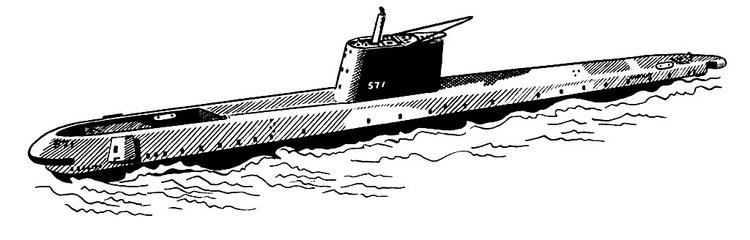
\includegraphics[width=4cm]{Q2-GK-AB.III.4-Abb_U-Boot.jpg}
	\end{wrapfigure}
	Ein militärisches U-Boot wurde von einer Beobachtungsstation im Punkt
	\punkt[U](1000|2000|-300) gesichtet (Angaben in \si{\meter} relativ zur
	Station). Laut Beobachtung bewegt es sich pro Minute um den Vektor
	$\vec{v} = \vector*(320|-250|55)$ fort.

	\begin{teilaufgaben}
		\teilaufgabe
		Bestimme die wahrscheinliche Position des U-Boots nach einer,
		zwei, dreieinhalb und fünf Minuten. Bestimme die Position relativ zum
		Ausgangspunkt $U$, sowie zur Beobachtungsstation (dem Koordinatenursprung).

		\teilaufgabe
		Skizziere die Punkte in einem Koordinatensystem mit geeignetem Maßstab.
		Verdeutliche dabei die Bewegung des U-Bootes.

		\teilaufgabe
		Stelle eine allgemeine Formel zur Berechnung des Ortsvektors $\vec{OX}$ der
		Position $X$ des U-Boots nach $t$ Minuten auf (relativ zu $U$ und zum Ursprung).
		Beschreibe dein vorgehen.

		\teilaufgabe\iconStern~
		Wann erreicht das U-Boot die Oberfläche und welche Position hat es zu diesem
		Zeitpunkt? Welche Strecke hat es dann von seinem Startpunkt zurück gelegt?
	\end{teilaufgaben}
\end{aufgabe}

\end{document}
